Nel secondo esperimento si vuole realizzare una semplice stazione di monitoraggio ambientale gestota dalla scheda Arduino Due che tramite un display TFT, riporta i dati da sensori analogici di umidità e temperatura e sensori digitali $I^2C$ di temperatura e luminosità. Per questo esperimento sono stati utilizzati i seguenti componenti:
\begin{itemize}
    \item Sensore di temperatura analogico, codice \textit{TMP36}, Analog Devices
    \item Sensore di umidità analogico, codice \textit{HIH-5030-001}, Honeywell
    \item Sensore di temperatura digitale, codice \textit{DS1621}, Maxim
    \item Sensore di luce ambientale, codice \textit{TSL2561}, TAOS
    \item Display TFT 3.5" 320x480, \textit{HX8357} Adafruit
    \item Scheda Arduino DUE, breadboard e cavi
    \item Interruttore e resistenza $R=10\text{ k}\Omega$
\end{itemize}
Il circuito è alimentato mediante porta USB del PC, la quale eroga circa $(\sim 5 V)$. La scheda Arduino due ha due bus $I^2C$, utilizzeremo i pin 20(SDA) e 21(SCL).
\begin{figure}[H]
    \centering
    \begin{minipage}{.5\textwidth}
      \centering
      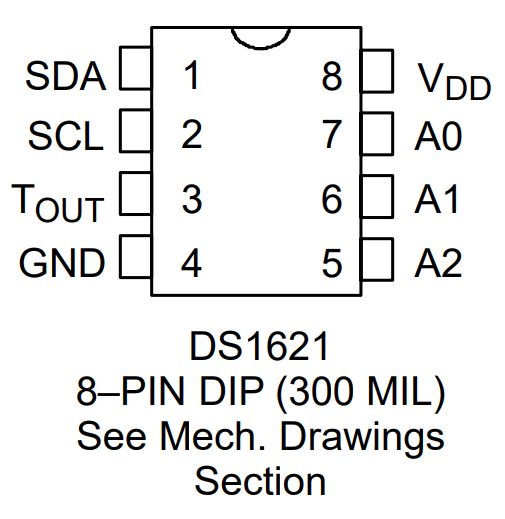
\includegraphics[width=.8\linewidth]{images/DS1621.png}
      \captionof{figure}{Pinout sensore DS1621}
      \label{fig:DS1621}
    \end{minipage}%
    \begin{minipage}{.5\textwidth}
      \centering
      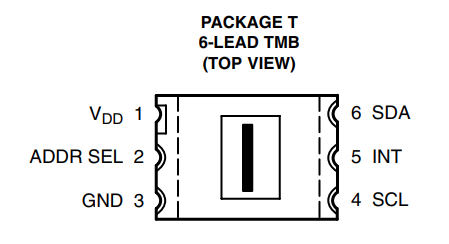
\includegraphics[width=\linewidth]{images/TSL2561.png}
      \captionof{figure}{Pinout sensore TSL2561}
      \label{fig:TSL2561}
    \end{minipage}
\end{figure}
Abbiamo collegato a GND i pin $A_0,A_1,A_2$ del sensore DS1621 in modo che il suo indirizzo sia \texttt{0x48}. Lasciando flottante il pin \texttt{ADDR SEL} del sensore TSL2561 il suo indirizzo è \texttt{0x39}.
\begin{figure}[H]
    \centering
    \begin{minipage}{.5\textwidth}
      \centering
      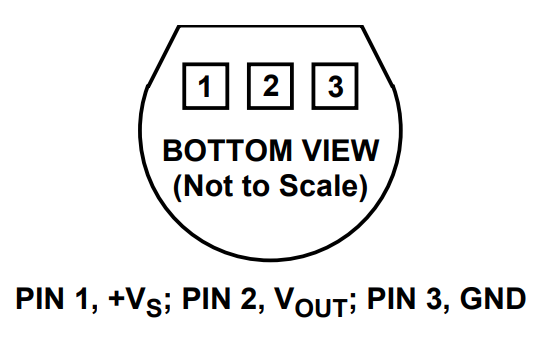
\includegraphics[width=.8\linewidth]{images/TMP36.png}
      \captionof{figure}{Pinout sensore TMP36}
      \label{fig:DS1621}
    \end{minipage}%
    \begin{minipage}{.5\textwidth}
      \centering
      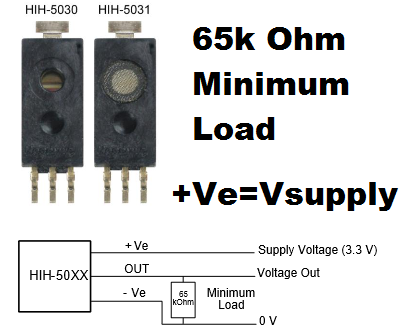
\includegraphics[width=.8\linewidth]{images/HIH-5030.png}
      \captionof{figure}{Pinout sensore HIH-5030}
      \label{fig:TSL2561}
    \end{minipage}
\end{figure}
\subsection{Codice - interfaccia grafica}
Per il funzionamento del Display HX8357 con Arduino è necessario importare le librerie \texttt{Adafruit\_HX8357.h}, \texttt{Adafruit\_GFX.h} e \texttt{SPI.h}. Per comunicare con i dispositivi $I^2C$ è necessario utilizzare la libreria \texttt{Wire.h}. 
\begin{lstlisting}[frame=single, language=Arduino]
#include <SPI.h>
#include <Wire.h>
#include "Adafruit_GFX.h"
#include "Adafruit_HX8357.h"

#define TEMP_DEV_ID 0x48
#define LIGHT_DEV_ID 0x39

#define HUMIDITY_DEV_PIN A1
#define TEMP_PIN A0

#define TFT_CS 10
#define TFT_DC 9

Adafruit_HX8357 tft = Adafruit_HX8357(TFT_CS, TFT_DC, -1); 
// TFT_RST set to -1 to tie it to Arduino's reset

#define buttonPin 2

bool pulsante_precedente_alto = LOW;
bool stateButton = LOW;
int stato = 0;
int stato_precedente = 0;

float temperatura_precedente_analog = 0;
\end{lstlisting}
\begin{lstlisting}[frame=single, language=Arduino]
void setup(){
    analogReadResolution(12);
    Wire.begin();

    // Configurazione del sensore di temperatura digitale DS1621
    Wire.beginTransmission(TEMP_DEV_ID); // Connect
    Wire.write(0xAC);   // Access config
    Wire.write(0x02);   // Set for continuos conversion
    Wire.endTransmission();

    Wire.beginTransmission(TEMP_DEV_ID);
    Wire.write(0xEE);   // Start conversion
    Wire.endTransmission();

    // Configurazione del sensore di luce digitale TSL2561
    Wire.beginTransmission(LIGHT_DEV_ID);
    Wire.write(0x00);   // Access Configuration options
    Wire.write(0x03);   // Sets power up
    Wire.endTransmission();

    Wire.beginTransmission(LIGHT_DEV_ID);
    Wire.write(0x81);   // Command to se timing
    Wire.write(0x02);   // Low Gain (1x), 402ms (default)
    Wire.endTransmission();

    // configurazione del Display TFT
    tft.begin();
    tft.setRotation(3);
    tft.fillScreen(HX8357_BLACK);
    tft.setTextSize(5);

    attachInterrupt(digitalPinToInterrupt(2),change_state,RISING);
}
\end{lstlisting}
Funzione interrupt necessaria per cambiare quale sensore si vuole visualizzare. 
\begin{lstlisting}[frame=single, language=Arduino]
void change_state(){
  stato++;
  if(stato >= 4)
    stato = 0;
}
\end{lstlisting}
\clearpage
\begin{lstlisting}[frame=single, language=Arduino]
void loop(){
    switch(stato){
        case 0:{
            if (stato != stato_precedente) {
              tft.fillScreen(HX8357_BLACK);
              tft.setCursor(30,60);
              tft.println("Temperatura 1");
            }
            float temp = AnalogTemperature(TEMP_PIN);
            String txt = String(temp);
            tft.setCursor(60,120);
            tft.fillRect(60,120,480,320, HX8357_BLACK);
            tft.println(txt + " C");
            stato_precedente = 0;
        }
        break;
        case 1:{
            if (stato != stato_precedente) {
              tft.fillScreen(HX8357_BLACK);
              tft.setCursor(30,60);
              tft.println("Temperatura 2");
            }
            float temp = DigitalTemperature();
            String txt = String(temp);
            tft.setCursor(60,120);
            tft.fillRect(60,120,480,320, HX8357_BLACK);
            tft.println(txt + " C");
            stato_precedente = 1;
        }
        break;
        case 2:{
            if(stato != stato_precedente) {
              tft.fillScreen(HX8357_BLACK);
              tft.setCursor(30,60);
              tft.println("Luminanza");
            }
        
            int lux = DigitalLight();
            String txt = String(lux);
            tft.setCursor(60,120);
            tft.fillRect(60,120,480,320, HX8357_BLACK);
            tft.println(txt + " lux");
            stato_precedente = 2;
        }
        break;
        case 3:{
            if (stato != stato_precedente) {
              tft.fillScreen(HX8357_BLACK);
              tft.setCursor(30,60);
              tft.println("Humidity");
            }
            float hum = AnalogHumidity(HUMIDITY_DEV_PIN);
            String txt = String(hum);
            tft.setCursor(60,120);
            tft.fillRect(60,120,480,320, HX8357_BLACK);
            tft.println(txt + " %");
            stato_precedente = 3;
        }
    }
    delay(500);
}
\end{lstlisting}
\subsection{Codice - lettura sensori}
Qui di seguito sono riportate le funzioni che leggono i dati dai vari sensori. Per le letture dai sensori analogici si è deciso di impostare il DAC di Arduino Due a 12 bit, in modo da avere una risoluzione maggiore con 4096 livelli.\\\\
Il sensore TMP36 restituisce in output una tensione proporzionale alla temperatura.
\begin{lstlisting}[frame=single, language=Arduino, caption = Lettura dal sensore TMP36, label = lst:AnalogTemp]
int AnalogTemperature(int pin) {
    float analogValue = analogRead(pin);
    float temperatura = (analogValue - 155) *330.0/4095.0; //12 bit DAC
    return temperatura;
}
\end{lstlisting}
Per ottenere il valore di umidità corretto è necessario modificare la lettura del sensore in base alla temperatura utilizzando le formule fornite dal datasheet del componente
\begin{lstlisting}[frame=single, language=Arduino, caption = Lettura dal sensore HIH-5030, label = lst:AnalogHum]
int AnalogHumidity(int pin) {
    float analogValue = analogRead(pin);
    float rhvoltage = (analogValue/4095.0)*3.3; // 12 bit DAC
    float umidita = ((rhvoltage/3.3)-0.1515)/0.00636;
    umidita = umidita/(1.0546-0.00216*AnalogTemperature(A0));
    return umidita;
}
\end{lstlisting}
\begin{lstlisting}[frame=single, language=Arduino]
int DigitalTemperature(){
    int firstByte, secondByte;
    float temp = 0;
    Wire.beginTransmission(DEV_ID);
    Wire.write(0xAA); // Temperature register   
    Wire.endTransmission();
    Wire.requestFrom(DEV_ID, 2); // request 2 bytes from slave device

    firstByte = Wire.read(); // read first byte
    secondByte = Wire.read(); // read second byte

    temp = firstByte;
    if(secondByte)  temp += 0.5;

    return temp;
}
\end{lstlisting}
\begin{lstlisting}[frame=single, language=Arduino]
int DigitalLight(){
    byte firstByte, secondByte;
    int lux = 0;

    Wire.beginTransmission(DEV_ID2);
    Wire.write(0x8C);   // Access LSB of ADC0
    Wire.endTransmission();
    Wire.requestFrom(DEV_ID2, 1);

    firstByte = Wire.read(); // read first byte

    Wire.beginTransmission(DEV_ID2);
    Wire.write(0x8D);   // Access MSB of ADC0
    Wire.endTransmission();
    Wire.requestFrom(DEV_ID2, 1);

    secondByte = Wire.read(); // read second byte

    lux = 256 * int(secondByte) + int(firstByte); 
    // convert the two bytes to int
    return lux;
}
\end{lstlisting}
E' possibile apprezzare il funzionamento del circuito dal video al \href{https://mediaspace.unipd.it/media/Esperimento+2/1_o92nu58e}{seguente link}